\documentclass[fleqn,10pt,lineno]{wlpeerj}\usepackage[]{graphicx}\usepackage[]{color}
%% maxwidth is the original width if it is less than linewidth
%% otherwise use linewidth (to make sure the graphics do not exceed the margin)
\makeatletter
\def\maxwidth{ %
  \ifdim\Gin@nat@width>\linewidth
    \linewidth
  \else
    \Gin@nat@width
  \fi
}
\makeatother

\definecolor{fgcolor}{rgb}{0.345, 0.345, 0.345}
\newcommand{\hlnum}[1]{\textcolor[rgb]{0.686,0.059,0.569}{#1}}%
\newcommand{\hlstr}[1]{\textcolor[rgb]{0.192,0.494,0.8}{#1}}%
\newcommand{\hlcom}[1]{\textcolor[rgb]{0.678,0.584,0.686}{\textit{#1}}}%
\newcommand{\hlopt}[1]{\textcolor[rgb]{0,0,0}{#1}}%
\newcommand{\hlstd}[1]{\textcolor[rgb]{0.345,0.345,0.345}{#1}}%
\newcommand{\hlkwa}[1]{\textcolor[rgb]{0.161,0.373,0.58}{\textbf{#1}}}%
\newcommand{\hlkwb}[1]{\textcolor[rgb]{0.69,0.353,0.396}{#1}}%
\newcommand{\hlkwc}[1]{\textcolor[rgb]{0.333,0.667,0.333}{#1}}%
\newcommand{\hlkwd}[1]{\textcolor[rgb]{0.737,0.353,0.396}{\textbf{#1}}}%

\usepackage{framed}
\makeatletter
\newenvironment{kframe}{%
 \def\at@end@of@kframe{}%
 \ifinner\ifhmode%
  \def\at@end@of@kframe{\end{minipage}}%
  \begin{minipage}{\columnwidth}%
 \fi\fi%
 \def\FrameCommand##1{\hskip\@totalleftmargin \hskip-\fboxsep
 \colorbox{shadecolor}{##1}\hskip-\fboxsep
     % There is no \\@totalrightmargin, so:
     \hskip-\linewidth \hskip-\@totalleftmargin \hskip\columnwidth}%
 \MakeFramed {\advance\hsize-\width
   \@totalleftmargin\z@ \linewidth\hsize
   \@setminipage}}%
 {\par\unskip\endMakeFramed%
 \at@end@of@kframe}
\makeatother

\definecolor{shadecolor}{rgb}{.97, .97, .97}
\definecolor{messagecolor}{rgb}{0, 0, 0}
\definecolor{warningcolor}{rgb}{1, 0, 1}
\definecolor{errorcolor}{rgb}{1, 0, 0}
\newenvironment{knitrout}{}{} % an empty environment to be redefined in TeX

\usepackage{alltt} % for journal submissions
\usepackage{hyperref}
% \documentclass[fleqn,10pt]{wlpeerj} % for preprint submissions

\title{Method for evaluating genomic material purity using whole genome sequencing data.}

\author[1]{Nathan D. Olson}
\author[1]{Justin Zook}
\author[1]{Jayne Morrow}
\author[1]{Nancy Lin}
\affil[1]{Biosystems and Biomaterials Division, National Institute of Standards and Technology}

\keywords{Biodetection, Test material, Reference material, Purity, Bioinformatics}

\begin{abstract}
Dummy abstract text. 

\end{abstract}
\IfFileExists{upquote.sty}{\usepackage{upquote}}{}
\begin{document}















\flushbottom
\maketitle
\thispagestyle{empty}

\section*{Introduction}
Rapid, sensitive and accurate assays for detecting bacterial pathogens in food, water, clinical samples, and  suspicious biothreats is critical to public health and safety. 
Biodetection assays must be evaluated for assay sensitivity and specificity prior to deployment as well in the hands of the user to instill confidence in the actions made based on assay results \citep{Ieven2013,International2011,EPA2004,ISO/TS2010,Guide1998,Feldsine2002}. 
Test materials are used to validate assay performance.  Test materials can be either purified cultures, genomic DNA or whole cells spiked into a matrix \citep{EPA2004,ISO/TS2010,CLSI2010}. 
Before being used to evaluate a biodetection assay the material itself must be validated in terms of purity and identity to eliminate false positive results due to test material contaminants or false negatives due to the test material being the wrong strain \citep{CLSI2010}. 
There are a number of potential sources of microbial contaminants  including the stock culture, preservation medium, as well as airborne and laboratory contaminants \citep{Marron2013,Shrestha2013,Tanner1998}.   
 
Currently polymerase chain reaction (PCR) assays are the most commonly use method for evaluating test material purity. 
Though other methods to detect contaminants in whole genome sequencing datasets have been developed but not currently used to evaluate test material purity.
A PCR assay was developed to analyze protist cultures. 
This assay uses endpoint PCR for prokaryotes and eukaryotes with template dilutions \citep{Marron2013}. 
The benefit to PCR-based approaches is that they can be cost effective and fast if an applicable protocol exists. 
While PCR assays can detect contaminants, this approach does not scale to multiple contaminants and test materials. 
More importantly, PCR assays can only target specific contaminants thus biases the purity assessment to known potential contaminants.
The bioinformatics tools developed to identify contaminants in metagenomic datasets, which include sequencing data from all organisms in a sample, can also be used to evaluate test material purity. 
For example DeconSeq \citep{Schmieder2011} and a similar method QC-Chain \citep{Zhou2013} were developed to identify contaminants based on analysis of 16S ribosomal ribonucleic acid (rRNA) gene sequences or comparison of a subset of reads to a reference database using Basic local alignment search tool (BLAST). 
Metagonomic-based methods are able to identify contaminants without any prior knowledge or assumptions regarding the identity of the organism(s). 
However, methods based on 16S rRNA gene identification have limited resolution, as 16S rRNA sequences can only provide genus level taxonomic resolution at best. 
 The benefit to using metagenomic tools developed is that prior knowledge of the identity of the contaminant is not required; however this method is unable to identify contaminants to the species level or higher.   

Another approach to evaluating test material purity is through shotgun whole genome sequencing, sequence all DNA in a single organism sample. 
There are a number of metagenomic read classification algorithms developed to determine the taxonomic composition of a sequence dataset of unknown composition. These algorithms tend to use one of three primary strategies for taxonomic assignment. The first method consist of aligning reads to an reference database\citep{buchfink2015fast, Francis2013}. This approach while exaustive is computationally expensive. 
The second type of method focuses on marker genes, genes common to different phylogenetic groups, which reduces the computational cost \citep{segata2012metagenomic, liu2011accurate}. 
The decrease in computational cost comes at a price at information required to discriminate closely related genomes may not be present in the marker genes.
The third method uses a $k$-mer based approach, where taxonomic composition is determined based the abundance of DNA sequences of length $k$ in the sequence dataset and a reference database \citep{ounit2015clark, menzel2016fast, wood2014kraken}. 

In this work, we present the results of a proof of concept study to measure the purity of single organism test materials using whole genome sequencing data combined with a metagenomic read classification algorithm. 
We choose to use \textit{Pathoscope}, a sequence alignment based method, 
developed use in detecting pathogens and identify strains using whole genome sequencing data \citep{Francis2013}, 
as the pathogen detection problem is similar to contaminant detection as the organism of interest is likely present at low concentrations. 
\textit{Pathoscope} benefits from the large sample size obtained using all sequence data for higher sensitivity(compared to marker gene based methods) and leverages algorithmic advances for whole genome sequence mapping. 
We will first present the specificity of the method using simulated data for single organisms. 
Then, evaluate sensitivity of the method using simulated contaminanted test material datasets.  


\section*{Methods}
To test the suitability of using whole genome sequence data and metagenomic taxonomic classification methods for evaluating material purity we first simulated whole genome sequence data from single genomes and also simulated contaminanted datasets. 
Simulated data from single genomes was used to assess method specificity and simulated contaminant datasets method sensitivity. Simulated datasets were generated using the ART sequencing read simulator \citep{Huang2012}. 
The datasets were generated using the Illumina MiSeq error models for 230 paired end base pair reads and 20 X mean coverage with an average insert size of 690 base pairs with standard deviation of 10 bp for each strain, 
the seed number for the random number generator was randomly assigned and recorded for each dataset. 

The taxonomic composition of simulated datasest was assessed using the Pathoscope metagenomic taxonomic classifier \citep{Francis2013}. 
This method uses an expectation maximization algorithm where the sequence data are first mapped to a database comprised on all sequence data in the Genbank nt database, 
then through an iterative process re-assigns ambiguously mapped reads to based on the proportion of reads mapped unambigously to individual taxa in the database. 
The PathoScope 2.0 taxonomic read classification pipeline includes an initial read filtering step (PathoQC), 
followed by mapping reads to a reference database (PathoMap) - a wrapper for bowtie2 \citep{Langmead2012}), then an expectation-maximization classification algorithm (PathoID). 
The annotated Genbank nt database provided by the PathoScope developers was used as the reference database (\url{ftp://pathoscope.bumc.bu.edu/data/nt\_ti.fa.gz}).

\subsection*{Specificity} 
Method specificity was defined as the proportion of reads in a single organism simulated dataset assigned to a different taxonomy then the taxonomy of the test material. 
Sequence data was simulated for 406 strains, from 9 genera (Table \ref{tab:single_org}). 
We will refer to the genome used to generate the reads as the target genome. 
The genomes included in the simulation study were limited to the number of closed genomes in the Genbank database (\url{http://www.ncbi.nlm.nih.gov/genbank/}, accessed 10/18/2013) belonging genera of interest (Table \ref{tab:single_org}). 
Due to the large number of closed genomes genomes from the genera \textit{Bacillus}, \textit{Escherichia}, and \textit{Salmonella} were limited to thefollow species \textit{Bacillus cereus}, \textit{Escherichia coli}, \textit{Salmonella enteria}. 
The taxononomic heirarchy for the target genome and simulated read assignment match levels were determined using the R package \citep{TaxizeArticle,TaxizeManual}. 

\subsection*{Sensitivity}
We simulated datasets with contaminants to evaluate method sensitivity. 
Representative genomes for 8 of the 9 genus were used to generate the simulated contaminant datasets (Table \ref{tab:contam_table}). 
An \textit{Escherichia coli} strain was selected as a representative of both \textit{Eschericha coli} and \textit{Shigella}. 
For each pairwise combination of representative genomes for the simulated contaminant dataset was subsampled at $0.1$ to $10^{-8}$ (contaminant proportion), at 10 fold dilutions, the target genome dataset was subsamples at 1 - contaminant proportion, resulting in 512 simulated contaminant datasets. 
This approach simulates the proportions of cells in a test material and not the amount of DNA, assuming unbiased DNA extraction. 
To speed up processing the aligned sequence files were subsampled instead of the simulated sequence files. 

\subsection*{Reproducibility}
To facility reproducibility and transparency a Docker (\url{www.docker.com}) container is available with installed pipeline dependencies (\url{www.registry.hub.docker.com/u/natedolson/docker-pathoscope/}). 
The script used to run the simulations were available at \url{https://github.com/nate-d-olson/genomic_purity}. 
Pathoscope results were processed using using the statistical programing language R \citep{R} and intermediate analysis and data summaries were organized using ProjectTemplate \citep{ProjectTemplate} and archived in a github repository (\url{https://github.com/nate-d-olson/genomic_purity_analysis}).

\section*{Results and Discussion}

\subsection*{Specificity}

Simulated sequence data from individual isolates was used to assess the genomic purity assessment method specificity.  
Here we define specificity as the ability of the method to correctly assign reads to the taxonomy of the genome the sequencing reads were simulated from, the target genome. 
Method specificity was evaluated by characterizing the read assignment results based on the level of agreement between the genome and assigned taxonomy (Fig. \ref{fig:single_org_cum}). 
Overall high proportion of matches at species and genus level. 
The cumulative match proportions do not always reach 1.00, for example \textit{Staphylococcus} genomes. 
This might be due to exclusion of unclassified and unknown matches (NCBI taxid 12908 and 0 respecitively) from match level analysis. 
Some genus have high levels of family and higher matches. 
For \textit{Shigella} most likely due to matches with \textit{Escherichia} (Fig. \ref{fig:shigella_ec_cum}). 

% latex table generated in R 3.3.0 by xtable 1.8-2 package
% Mon Jul 11 21:50:18 2016
\begin{table}[ht]
\centering
\begin{tabular}{lrl}
  \hline
Genus & N & Genome Size (Mb) \\ 
  \hline
\textit{Bacillus} &  76 & 5.05 (3.07-7.59) \\ 
  \textit{Escherichia} &  62 & 5.11 (3.98-5.86) \\ 
  \textit{Pseudomonas} &  57 & 6.18 (4.17-7.01) \\ 
  \textit{Staphylococcus} &  49 & 2.82 (2.69-3.08) \\ 
  \textit{Salmonella} &  44 & 4.88 (4.46-5.27) \\ 
  \textit{Listeria} &  39 & 2.97 (2.78-3.11) \\ 
  \textit{Clostridium} &  32 & 4.02 (2.55-6.67) \\ 
  \textit{Yersinia} &  19 & 4.73 (4.62-4.94) \\ 
  \textit{Francisella} &  18 & 1.89 (1.85-2.05) \\ 
  \textit{Shigella} &  10 & 4.74 (4.48-5.22) \\ 
   \hline
\end{tabular}
\caption{Breakdown of the number of genomes by genus used to generate single genome simultated datasets. N indicates the number of genomes, and Genome Size is presented as the median and range (minimum to maximum) genome size} 
\label{tab:single_org}
\end{table}


\begin{knitrout}
\definecolor{shadecolor}{rgb}{0.969, 0.969, 0.969}\color{fgcolor}\begin{figure}

{\centering 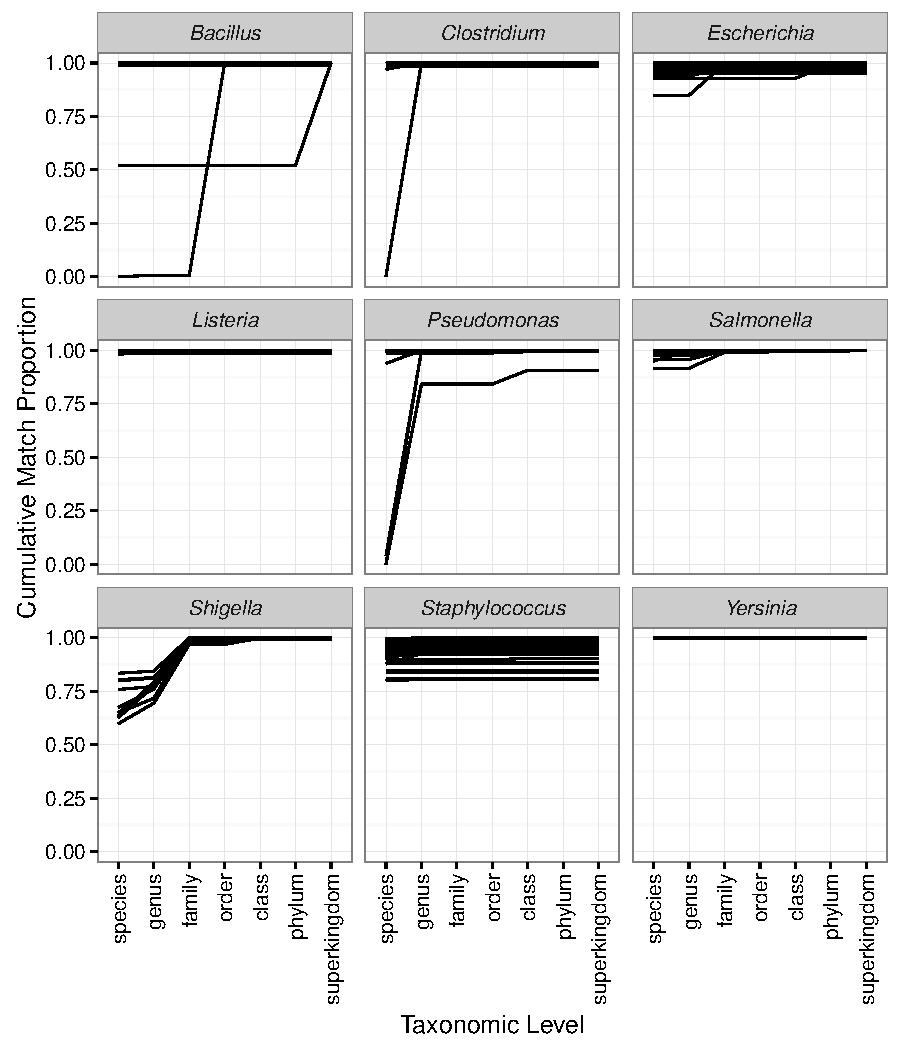
\includegraphics[width=\maxwidth]{figure/single_org_cum-1} 

}

\caption[Cumulative taxonomic match results for genomic purity assements of simulated sequence data from single genomes]{Cumulative taxonomic match results for genomic purity assements of simulated sequence data from single genomes.  Each line represents the cumulative proportion of simulated reads with taxonomic assignments matching at or above the specified taxonomic level. Genomes are grouped by genus.}\label{fig:single_org_cum}
\end{figure}


\end{knitrout}


\begin{knitrout}
\definecolor{shadecolor}{rgb}{0.969, 0.969, 0.969}\color{fgcolor}\begin{figure}

{\centering 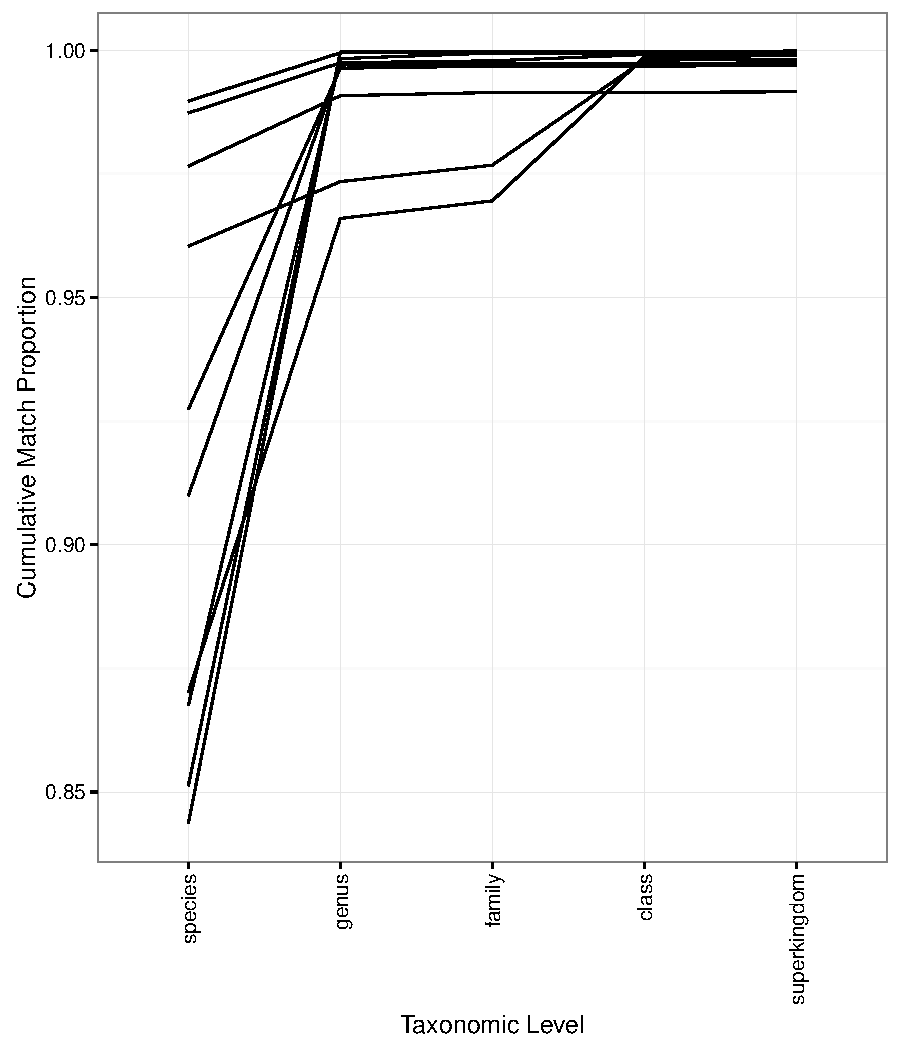
\includegraphics[width=\maxwidth]{figure/shigella_ec_cum-1} 

}

\caption{Cumulative taxonomic match results for genomic purity assement for \textit{Shigella} considering matches to \textit{E. coli} as species level matches.  Each line represents the cumulative proportion of simulated reads with taxonomic assignments matching at or above the specified taxonomic level. Genomes are grouped by genus.}\label{fig:shigella_ec_cum}
\end{figure}


\end{knitrout}

Most of the genus had genus level or higher match proportions excluding a few outliers (Fig. \ref{fig:single_genus}). 
\textit{Escherichia}, \textit{Shigella}, and \textit{Staphylococcus} are noteable exceptions. 
As discussed previously the taxonomic ambiguities for \textit{Shigella} and \textit{Escherichia} are responsible for the overall lower genus level match proportions. Another example of low genus level matches is the \textit{Bacillus} genome with genus match proportion close to zero, \textit{Bacillus infantis} string NRRL B 14911. While the \textit{B. infantis} strain was originally classified as \textit{Bacillus} the species is phylogenetically distinct from other members of the genus \citep{ko2006bacillus}.
It is important to consider the strain and genome being characterized as taxonomic ambiguities (e.g. \textit{Shigella} and \textit{Escherichia}) can lead to lower than expected specificity and the identification of false positive contaminants.  


\begin{knitrout}
\definecolor{shadecolor}{rgb}{0.969, 0.969, 0.969}\color{fgcolor}\begin{figure}
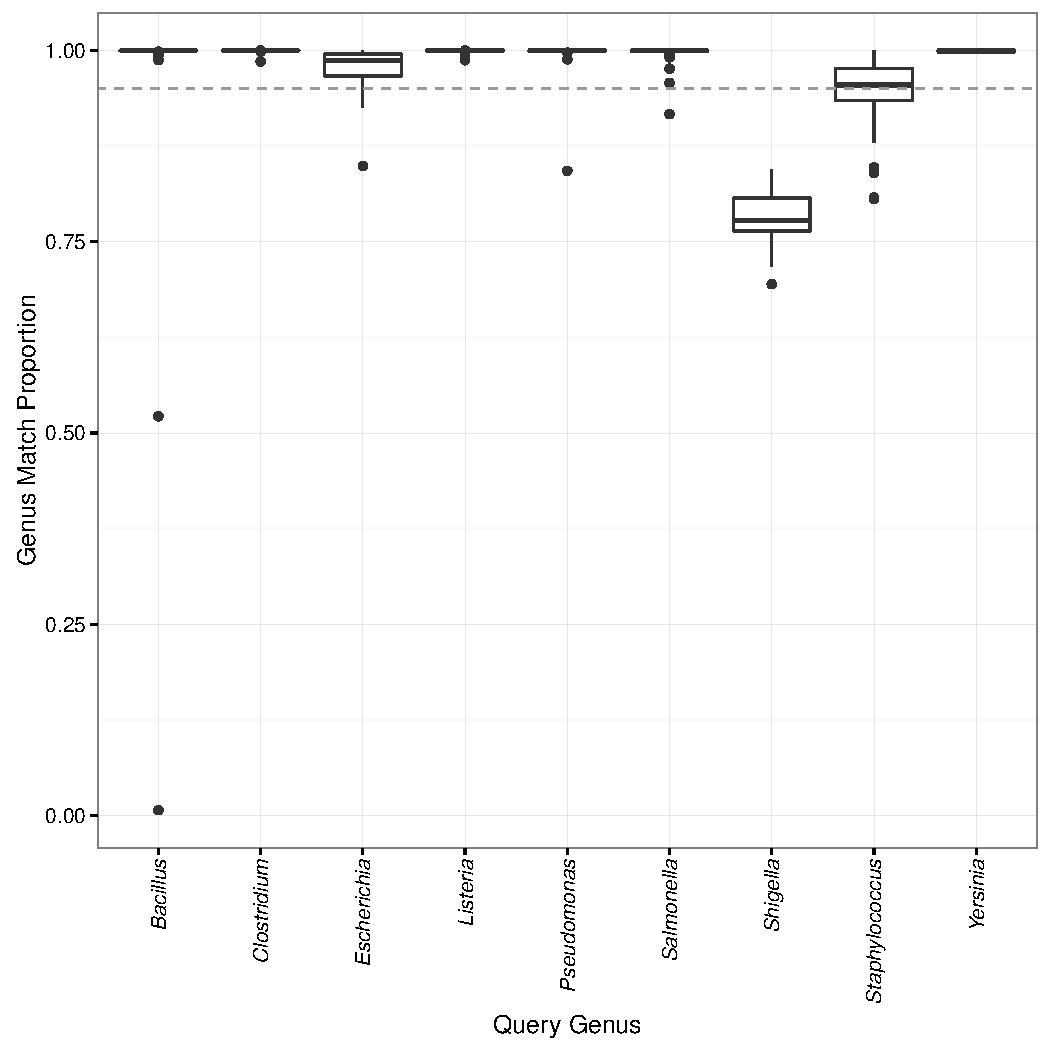
\includegraphics[width=\maxwidth]{figure/single_genus-1} \caption[Distribution of the proportion of reads assigned to the source genome at or above the genus level]{Distribution of the proportion of reads assigned to the source genome at or above the genus level. Horizontal grey line highlights a match proportion of 0.95. Boxplots hinges represent the 25th and 75th percentiles, line through box represent is the median, whiskers are the 95\% confidence interval, and the black dots are outliers.}\label{fig:single_genus}
\end{figure}


\end{knitrout}

\subsection*{Sensitivity}
To evaluate genomic purity assessment methods we generated simulated contaminant datasets as pairwise combinations of representative genomes from 8 of the genus used in the specificity section of the study (Table \ref{tab:contam_table}). Due to the overall high proportion of reads matched to the correct genome in the method specificity study the simulated contaminant datasets were evaluated at the genus level. For all the uncontaminated representative set of target genomes the proportion of simulated reads that matched at species level or higher was 0.98 (Table \ref{tab:contam_table}).

% latex table generated in R 3.3.0 by xtable 1.8-2 package
% Mon Jul 11 21:50:19 2016
\begin{table}[ht]
\centering
\scalebox{0.65}{
\begin{tabular}{lrllll}
  \hline
Representative Strain & Species & C Mb & C Acc & P Mb & P Acc \\ 
  \hline
Bacillus anthracis str. Ames & 1.00 & 5.23 & AE016879.1 &  &  \\ 
  Clostridium botulinum A str. Hall & 1.00 & 3.76 & CP000727.1 &  &  \\ 
  Escherichia coli O157:H7 str. EC4115 & 0.98 & 5.57 & CP001164.1 & 0.13 & CP001163.1, CP001165.1 \\ 
  Francisella tularensis subsp. tularensis SCHU S4 & 1.00 & 1.89 & AJ749949.2 &  &  \\ 
  Pseudomonas aeruginosa PAO1 & 1.00 & 6.26 & AE004091.2 &  &  \\ 
  Salmonella enterica subsp. enterica serovar Typhimurium str. D23580 & 1.00 & 4.88 & FN424405.1 &  &  \\ 
  Staphylococcus aureus subsp. aureus ED133 & 0.98 & 2.83 & CP001996.1 &  &  \\ 
  Yersinia pestis CO92 & 1.00 & 4.65 & AL590842.1 & 0.18 & AL109969.1, AL117189.1, AL117211.1 \\ 
   \hline
\end{tabular}
}
\caption{Represenative strains used in simulated contaminant datasets. Species indicates the proportion of simulated reads assigned to the correct taxa at the species level or higher. DNA size (Mb) and Genbank accession numbers (Acc) are indicated for chromosomes (C) and plasmids (P). Escherichia coli O157:H7 str. EC4115 and Yersinia pestis CO92 have two and three plasmids respecitively.} 
\label{tab:contam_table}
\end{table}


While the proportion of contaminant reads in the simulated datasets was not equal to defined contaminant proportion the proportion of reads assigned to the contaminant genus was comparable to the expected proportion (Fig. \ref{fig:contam_min}). This was especially true for datasets containing mixtures of \textit{B. anthracis}, \textit{Y. pestis}, \textit{E. coli}, and \textit{S. enteria} as they had similar sized genomes (Table \ref{tab:contam_table}).  Three contaminants were detected when spiked in at contaminant proportions of $10^{-8}$, \textit{B. anthracis} in \textit{E. coli} as well \textit{S. enteria} and \textit{E. coli} in \textit{Y. pestis}. 
Interestingly the proportion of assigned reads did not decrease with decreasing contaminant proportions after $10^{-4}$. 

The lowest proportion of simulated contaminant detected varied by both contaminant and taget genome. 
All organisms had comparable minimum contamination levels for which reads were assigned to the contaminat genome. 
Two notable exceptions are \textit{Escherichia} and \textit{Yersinia}, where \textit{Bacillus}, and \textit{Salmonella} and \textit{Escherichia} were detected at the lowest contaminant levels respectively. 
As the results are from simulated data and based on proportions of simulated reads, these values do not indicate a limit of dection for the method.

\begin{knitrout}
\definecolor{shadecolor}{rgb}{0.969, 0.969, 0.969}\color{fgcolor}\begin{figure}
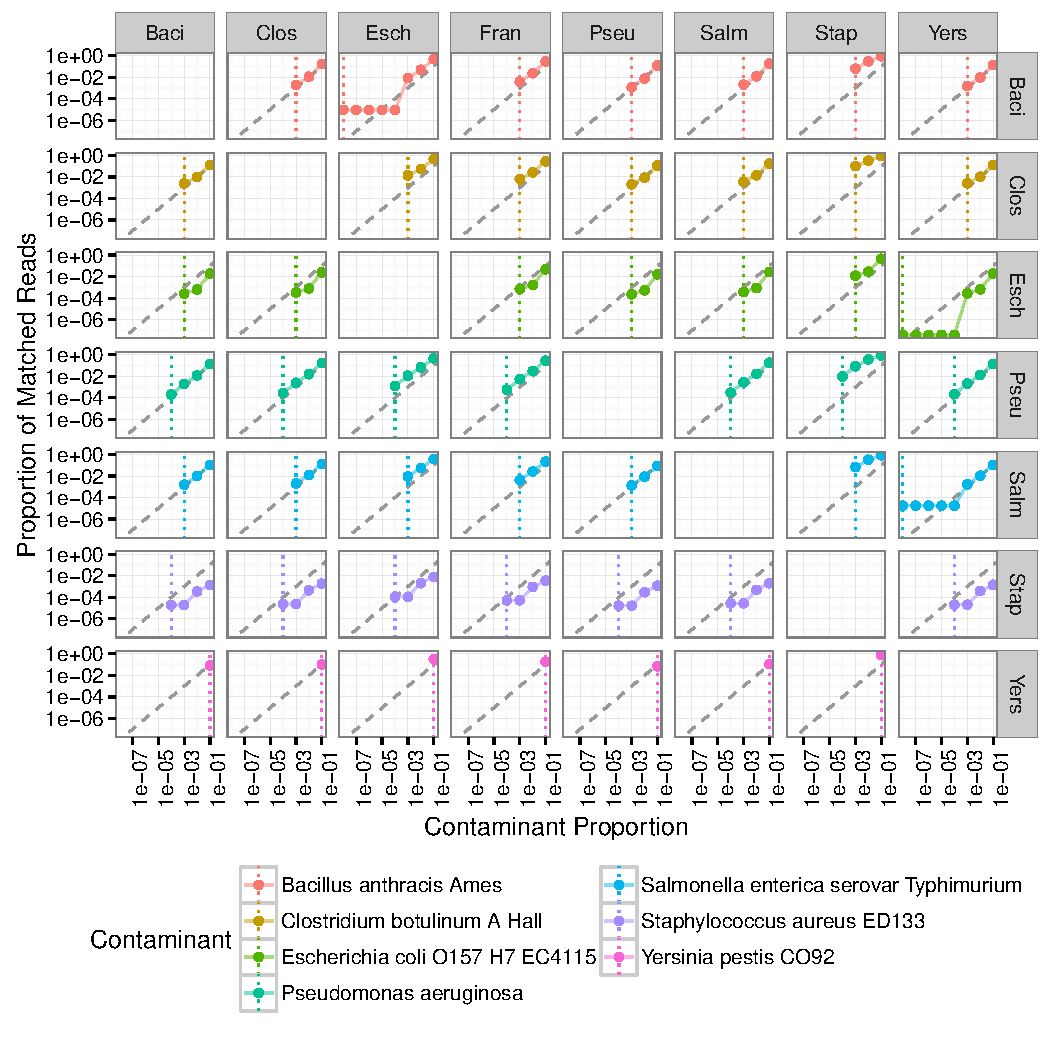
\includegraphics[width=\maxwidth]{figure/contam_min-1} \caption[Relationship between the proportion of contaminant reads simulated per dataset and the proportion of reads matched to the contaminant genus]{Relationship between the proportion of contaminant reads simulated per dataset and the proportion of reads matched to the contaminant genus.}\label{fig:contam_min}
\end{figure}


\end{knitrout}

\section*{Conclusions}  
\begin{itemize}
      \item Proof of concept study additional work required to validate use in assessing the purity of a test material.  
      \item Use of other taxonomic classification methods are likely to have different sensitivity and specificity results.
      \item Need to evaluate the suitablility of the reference database for used the genome and contaminant of interest.
      \item Work to further expand the taxonomic database to include genomes from uncultured organism using either metagenome datasets for single cell datasets along with efforts to address issues related to taxnomic ambiguities will help to improve the method applicability. 
\end{itemize}

\newpage

\section*{Acknowledgments}

The authors would like to thanks Dr. Steven Lund for his assistance in developing the study. 
The Department of Homeland Security (DHS) Science and Technology Directorate supported this work under the Interagency Agreement HSHQPM-12-X-00078 with the National Institute of Standards and Technology (NIST). 
Opinions expressed in this paper are the authors’ and do not necessarily reflect the policies and views of DHS,  NIST, or affiliated venues. 
Certain commercial equipment, instruments, or materials are identified in this paper in order to specify the experimental procedure adequately. 
Such identification is not intended to imply recommendations or endorsement by NIST, 
nor is it intended to imply that the materials or equipment identified are necessarily the best available for the purpose. 
Official contribution of NIST; not subject to copyrights in USA.

\bibliography{genomic_purity}

\end{document}
